\section{Introduction}\label{sec:intro}

The Large Hadron Collider (LHC) is created to explore the fundamental properties
of matter for the next decades. Since LHC start-up in 2009, the experiments
collected and distributed hundreds of petabytes of data worldwide to hundreds of
computer centers. Thousands of physicists analyze petascale data volumes daily.
One of the LHC experiments, the ATLAS~\cite{Aad:2008}, utilizes the Production
and Distributed Analysis (PanDA) workload management system~\cite{Maeno2011}
(WMS) for distributed data processing and analysis. The ATLAS Computing
model~\cite{Atlas2005} is based on a Grid paradigm~\cite{Foster:1998}, with
multilevel, hierarchically distributed computing and storage resources. PanDA
has been developed to meet growing ATLAS production and analysis requirements
for a data-driven workload management system capable of operating at LHC data
processing scale.

PanDA has a highly scalable architecture. Scalability has been demonstrated in
ATLAS through the rapid increase in usage over the past several years of
operations, and PanDA is expected to meet the continuously growing computing
requirements of ATLAS over the next decade. PanDA was designed to have the
flexibility to adapt to emerging computing technologies in processing, storage,
networking as well as the underlying software stack. This flexibility has also
been successfully demonstrated through the past six years: computing centers in
ATLAS, spanning many continents, were seamlessly integrated into PanDA\@.

PanDA manages a wide spectrum of workloads, ranging from raw data processing to
Monte Carlo simulation and user analysis, while constantly evolving to meet
rapidly changing science needs. Today, PanDA serves several thousand users,
managing job distribution to hundreds of ATLAS sites with more than 100,000 CPU
cores which process more than a million jobs per day (Figure~\ref{fig:daily}).

\begin{figure}
    \begin{center}
        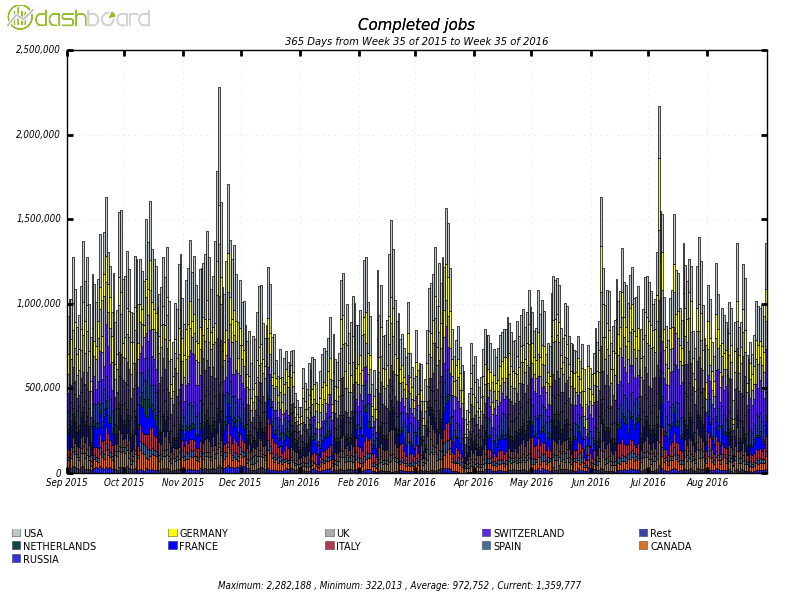
\includegraphics[width=\columnwidth]{figures/DailyJobs.png}
        \caption{Daily completed jobs on ATLAS Grid for the past 12 month}
    \end{center}
\label{fig:daily}
\end{figure}

In this paper, we describe how PanDA has been engineered to execute a specific
stage of the ATLAS Monte Carlo workflow on Titan, the larger high-performance
computing HPC system currently available in the USA\@.\mtnote{Explain the
benefits offered by Titan in terms of multithreading per node and possibly large
amount of concurrent nodes. Introduce also the notion of backfill.} This extends
the scope of PanDA's compute model, integrating both high-throughput and
high-performance computing resources and enabling the concurrent execution of
both  single and multi-core jobs. The integration of PanDA and Titan went
through three main engineering phases: (i) feasibility study and rapid
prototyping of an initial solution; (ii) progressing scaling of the  prototype
to saturate the available resources; (iii) study of a product-grade architecture
for generic HPC resources. Both phase i and ii have been completed enabling the
execution of up to eight million jobs a week on Titan. A prototype has been
engineered to support phase iii and experimental data are being collected.

In the next section we introduce \ldots.

Why Titan?
\begin{itemize}
    \item A lot of slow (relative the grid) and homogeneous cores together
    \item Grid is saturated
    \item Enable HPC as a calss of computing resource
    \item Enable future DOE experimental and observational capabilities on HPC
    \item Why is so important: more data, run 2 and run 3.
    \item growth of grid is flat (economic model) and saturated. We need more CPU because we have more data.
    \item ATLAS spend most of the time on simulations this is why we want to offload simulations - that happen happen to be performed via AthenaMP.
\end{itemize}
